\section{Definite Integrals \& Antiderivatives}

\subsection{Definition of a Definite Integral}
We saw several approximations for the areas under any type of curve.
We also saw how these approximations get better the narrower our ``strips''.
In the limit, we get exactly the area under the curve, which defines the definite integral.

\begin{definition}
	Let $f$ be continuous on the closed interval $[a,b]$.
	Let this interval be partitioned into $n$ equal\footnote{Technically, the intervals don't need to be of equal size, as long as the width of all intervals goes to 0 in the limit.} sub-intervals, each of length $\Delta x = \frac{b-a}{n}$.
	The definite integral of $f$ over $[a,b]$ is given by
	\begin{equation*}
		\int_{a}^{b}{f(x)\mathrm{d}x} = \lim_{n\to \infty}{\sum_{k=0}^{n-1}{f(c_k)\Delta x}}
	\end{equation*}
	where $c_k$ is any arbitrary value in the $k$th sub-interval.
	This particular type of limit of a sum is called a Riemann Sum.
\end{definition}

Note that the left, right, and midpoint approximations are all different ways of choosing $c_i$, all of which in the limit give the area under the curve and definite integral from $a$ to $b$.

\begin{example}
	Find the value of the following definite integral using Riemann sums.
	\begin{equation*}
		\int_{0}^{1}{x^2\d{x}}.
	\end{equation*}
\end{example}
\begin{answer}
	We'll use a Riemann sum with a left-endpoint approximation.
	\begin{align*}
		\int_{0}^{1}{x^2\d{x}} &= \lim_{n\to\infty}{\sum_{k=0}^{n-1}{f\left(0+\frac{k}{n}\right)\frac{1-0}{n}}} \\
		&= \lim_{n\to\infty}{\sum_{k=0}^{n-1}{\left(\frac{k}{n}\right)^2\frac{1}{n}}} \\
		&= \lim_{n\to\infty}{\sum_{k=0}^{n-1}{\frac{k^2}{n^3}}} \\
		&= \lim_{n \to \infty}{\frac{1}{n^3}\left(\frac{n(n-1)(2n-1)}{6}\right)} \\
		&= \lim_{n\to\infty}{\frac{1}{6}\left(2-\frac{3}{n}+\frac{1}{n^2}\right)} \\
		&= \frac{1}{3}.
	\end{align*}
\end{answer}


Note that area below the $x$-axis is counted as negative area.
In general
\begin{equation*}
	\int_{a}^{b}{f(x)\d{x}} = \text{ area above $x$-axis } - \text{ area below $x$-axis}.
\end{equation*}

\subsection{Basic Properties of Definite Integrals}
The following are properties of definite integrals.
Many should look familiar from properties of limits and derivatives.
Let $f$ and $g$ be continuous functions of $x$.
Let $a$, $b$, and $c$ be real constants where $a \neq b$.
Let $f_{[a,b]}$ be the values of $f$ on the interval $[a,b]$.
\begin{align*}
	\textbf{Order of Integration Rule: }& \int_{a}^{b}{f(x)\d{x}} = -\int_{b}^{a}{f(x)\d{x}} \\
	\textbf{Sum and Difference Rule: }& \int_{a}^{b}{(f(x) \pm g(x))\d{x}} = \int_{a}^{b}{f(x)\d{x}} \pm \int_{a}^{b}{g(x)\d{x}} \\
	\textbf{Zero Rule: }& \int_{a}^{a}{f(x)\d{x}} = 0 \\
	\textbf{Constant Multiple Rule: }& \int_{a}^{b}{cf(x)\d{x}} = c\int_{a}^{b}{f(x)\d{x}} \\
	\textbf{Additivity Rule: }& \int_{a}^{b}{f(x)\d{x}} + \int_{b}^{c}{f(x)\d{x}} = \int_{a}^{c}{f(x)\d{x}} \\
	\textbf{Max-Min Rule: }& (b-a)\min{f_{[a,b]}} \leq \int_{a}^{b}{f(x)\d{x}} \leq (b-a)\max{f_{[a,b]}} \\
	\textbf{Domination Rule: }& \min{f_{[a,b]}} \geq \max{g_{[a,b]}} \implies \int_{a}^{b}{f(x)\d{x}} \geq \int_{a}^{b}{g(x)\d{x}}.
\end{align*}

\subsubsection{Mean Value Theorem for Definite Integrals}
The mean value of $f$ over the interval $[a,b]$ is given by
\begin{equation*}
	\frac{1}{b-a}\int_{a}^{b}{f(x)\d{x}}.
\end{equation*}
You can effectively think of this as the definition of the average: adding up all the values and dividing by the number of values.
This is exactly what happens if you work through the Riemann sums.
Much like the Mean Value Theorem for Derivatives, since the function is continuous, it will take on its average value somewhere in the interval.
\begin{theorem}[Mean Value Theorem for Definite Integrals]
	If $f$ is continuous on the interval $[a,b]$, then there is some point $c$ in the interval such that
	\begin{equation*}
		f(c) = \frac{1}{b-a}\int_{a}^{b}{f(x)\d{x}}.
	\end{equation*}
\end{theorem}

\begin{figure}[H]
	\label{mvt_integrals}
	\centering
	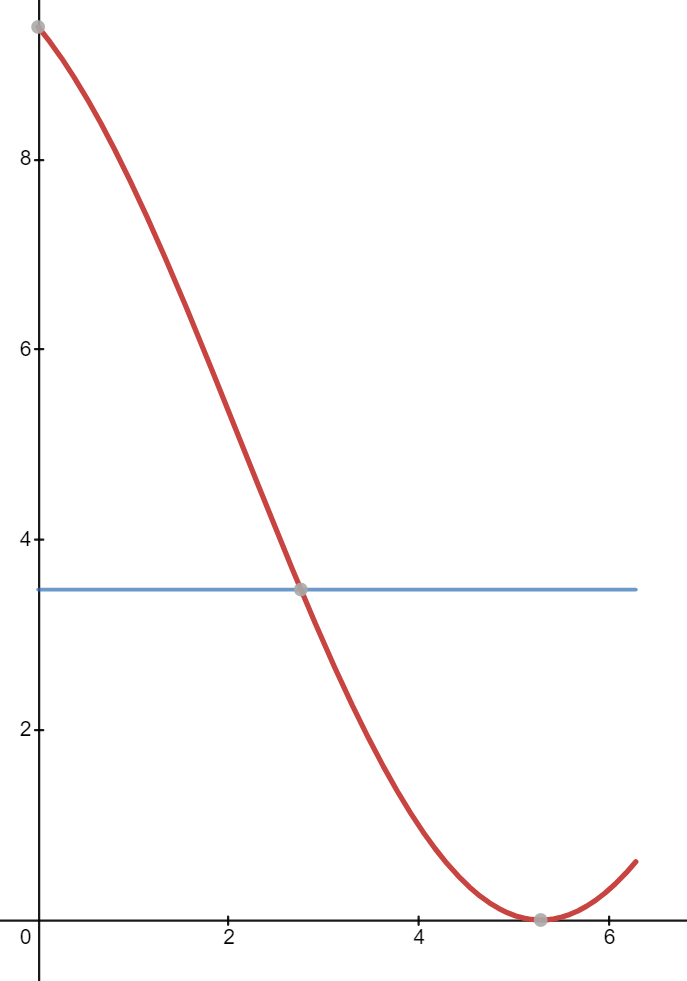
\includegraphics[width = 0.33\textwidth]{./integrals/mvt.png}
	\caption{A continuous function always takes on its mean value}
\end{figure}

\begin{example}
	A plane's airspeed is given by $v(t) = t/8\text{, }t\geq 0$.
	What what time $t$ does the Mean Value Theorem guarantee that the plane's speed was 1?
	When is this time?
\end{example}
\begin{answer}
	Rather than go through the trouble of evaluating a limit to find the definite integral, we can notice that the graph of the plane's airspeed is a triangle, which we know how to find the area of geometrically.
	\begin{equation*}
		\text{Area}(t) = \frac{1}{2}t v(t).
	\end{equation*}
	
	Dividing by the length of the interval to get the average airspeed,
	\begin{equation*}
		\text{Avg}(t) = \frac{1}{t-0}\hspace{3pt}\frac{1}{2}tv(t) = \frac{1}{2}v(t).
	\end{equation*}
	
	Solving for $t$ when $\text{Avg}(t)=1$,
	\begin{equation*}
		\frac{1}{2}\hspace{3pt}\frac{t}{8} = 1 \implies t = 16.
	\end{equation*}
	
	So, at time $t=16$, the Mean Value Theorem tells us that the plane's speed was 1.
	Looking at the graph, we can see that at time $t=8$ the plane's speed was indeed 1.
\end{answer}

\subsection{Fundamental Theorem of Calculus}
Although it's nice to be able to evaluate definite integrals for numerical bounds, it'd be more convenient if we only had to do the work of integrating once and could then have a function that would tell us the area like so:
\begin{equation*}
	F(x) = \int_{a}^{x}{f(t)\d{t}}.
\end{equation*}
Let's try taking the derivative of $F$ using the limit definition.
\begin{align*}
	F^\prime(x) &= \lim_{\Delta x \to 0}{\frac{F(x+\Delta x)-F(x)}{\Delta x}} \\
	&= \lim_{\Delta x\to 0}{\frac{\int_{a}^{x+\Delta x}f(t)\d{t} - \int_{a}^{x}{f(t)\d{t}}}{\Delta x}} \\
	&= \lim_{\Delta x\to 0}{\frac{\int_{x}^{x+\Delta x}{f(t)\d{t}}}{\Delta x}}\text{ (by Integral Rules)}\\
	&= \lim_{\Delta x\to 0}{\frac{f(k)\Delta x}{\Delta x}}\text{, }x\leq k \leq x + \Delta x\text{ (by Mean Value Theorem)} \\
	&= \lim_{\Delta x\to 0}{f(k)} \\
	&= f(x) \text{ (by Sandwich Theorem)}.
\end{align*}
Taking the derivative seems to undo the integration.
The same fact applies if we take the integral of a derivative.
Starting with what we've just shown,
\begin{equation*}
	\dd{}{x}\int_{0}^{x}{f(t)\d{t}} = f(x).
\end{equation*}
Let $g(x) = \dd{}{x}f(x)$.
\begin{equation*}
	\dd{}{x}\int_{0}^{x}{g(t)\d{t}} = g = \dd{}{x}f(x).
\end{equation*}
Since the derivatives are equal, we know the functions must differ by at most a constant $C$.
\begin{align*}
	\int_{0}^{x}{g(t)\d{t}} &= f(x) + C \\
	\int_{0}^{x}{\left[\dd{}{x}f(t)\right]\d{t}} &= f(x) + C.
\end{align*}
So, the integral of the derivative gets us a function that differs from the original by at most a constant.


This idea that the integral and derivative undo each other is captured by the Fundamental Theorem of Calculus.
\begin{theorem}[Fundamental Theorem of Calculus]
	Let $f$ be a continuous function on the interval $[a,b]$.
	Then
	\begin{equation*}
		F(x) = \int_{a}^{x}{f(t)\d{t}}
	\end{equation*}
	has a derivative at every point in $[a,b]$, and
	\begin{equation*}
		\dd{F}{x} = \dd{}{x}\int_{a}^{x}{f(t)\d{t}} = f(x).
	\end{equation*}
	Further, if $F$ is the antiderivative of $f$ on $[a,b]$, then
	\begin{equation*}
		\int_{a}^{b}{f(x)\d{x}} = F(b) - F(a).
	\end{equation*}
\end{theorem}

This last equation is especially useful for calculating definite integrals.
Rather than evaluating a limit of a Riemann sum, if we know the antiderivative, we can just evaluate at two points.

\begin{example}
	Evaluate the following definite integral using antiderivatives.
	\begin{equation*}
		\int_{0}^{1}{\frac{\d{x}}{1+x^2}}.
	\end{equation*}
\end{example}
\begin{answer}
	We previously derived that the derivative of $\arctan{x}$ is $\frac{1}{1+x^2}$.
	So, $\arctan{x}$ is the antiderivative of $\frac{1}{1+x^2}$.
	Applying the Fundamental Theorem of Calculus (FTC),
	\begin{align*}
		\int_{0}^{1}{\frac{\d{x}}{1+x^2}} &= \arctan{1} - \arctan{0} \\
		&= \frac{\pi}{4} - 0 \\
		&= \frac{\pi}{4}.
	\end{align*} 
\end{answer}

\subsection{Integrals of Symmetric Functions}
Suppose f is continuous on $[-a, a]$. Then we have
\begin{equation*}
	\int_{-a}^{a}{f(x)\d{x}} = 2 \int_{0}^{a}{f(x)\d{x}}
\end{equation*}
if f is even and
\begin{equation*}
	\int_{-a}^{a}{f(x)\d{x}} = 0
\end{equation*}
if f is odd.\bigskip

\noindent
Intuitively, since even functions are symmetric about the $y$-axis, it should make sense that the area under the curve from $-a$ to $a$ should be twice the area under the curve from 0 to $a$. 
Likewise, odd functions are symmetric about the origin, so any area under the curve above the $x$-axis will be canceled out by some corresponding area underneath the $x$-axis on the opposite side of the axis.

\begin{example}
	Evaluate the following definite integral.
	\begin{equation*}
		\int_{-1}^{1}{\frac{\tan{x}}{1 + x^2 + x^4}\d{x}}
	\end{equation*}
\end{example}
\begin{answer}
	At first, this looks like a nasty integral to evaluate. 
	However, we notice that $f(-x) = -\frac{\tan{x}}{1 + x^2 + x^4}$.
	Since $f(-x) = -f(x)$, the function is odd, and since the limits of integration are additive inverses of one another, we have
	\begin{equation*}
		\int_{-1}^{1}{\frac{\tan{x})}{1 + x^2 + x^4}} = 0.
	\end{equation*}
\end{answer}